%% In the documentclass line, replace "noanswers" with "answers" to view the key.

\documentclass[noanswers]{exam}
\usepackage[utf8]{inputenc}

\title{Chapter 3 Practice Problems}
\author{Sections 3.4--3.5}
\date{STAT 2300}

\usepackage[bottom=2.2cm, left=2.2cm, right=2.2cm, top=2.2cm]{geometry}
%\usepackage[paperheight=11in, paperwidth=17in, margin=1in]{geometry}
\usepackage{dsfont}
\usepackage{amsmath}
\usepackage{amssymb}
\usepackage{amsthm}
\usepackage{array}
\usepackage{stmaryrd}
\usepackage{pgfplots}
\pgfplotsset{width=10cm,compat=1.9}
\usepackage{multicol}
\setlength{\columnsep}{1in}
\usepackage{nicefrac}

\usepackage{multirow}
\usepackage{enumitem}[shortlabels]
\usepackage{tabu}
\definecolor{purp}{RGB}{102,0,204}
\usepackage{tabularx}
\newcolumntype{C}{>{\centering\arraybackslash $}X<{$}}
\usepackage{wrapfig}
\usepackage[export]{adjustbox}


\makeatletter
\pagestyle{headandfoot}
\firstpageheader{\@date}{\@title}{\@author}
\firstpageheadrule
\runningfootrule
\runningfooter{}{\thepage\ / \numpages}{\@title}
\makeatother

\newcommand{\abs}[1]{\left|#1\right|}
\newcommand{\mat}[4]{\left( \begin{tabular}{>{$}c<{$} >{$}c<{$}} #1&#2 \\ #3&#4 \end{tabular} \right)}
\newcommand{\msc}[1]{\mathds{#1}}
\newcommand{\Z}{\mathds{Z}}
\newcommand{\R}{\mathds{R}}
\newcommand{\N}{\mathds{N}}
\newcommand{\Q}{\mathds{Q}}
\newcommand{\C}{\mathds{C}}
\newcommand{\so}{\implies}
\newcommand{\set}[2]{\left\{ #1 \:|\: #2 \right\}}
\newcommand{\bso}{\Longleftarrow}
\newcommand{\ra}{\rightarrow}
\newcommand{\gen}[1]{\left\langle #1 \right\rangle}
\newcommand{\olin}[1]{\overline{#1}}
\newcommand{\Img}[1]{\text{Im}\left(#1\right)}
\newcommand{\llra}{\longleftrightarrow}
\newcommand{\lra}{\longrightarrow}
\newcommand{\xra}[1]{\xrightarrow{#1}}
\newcommand{\wo}{\setminus}
\newcommand{\mcal}[1]{\mathcal{#1}}
\newcommand{\Aut}[1]{\text{Aut}\left(#1\right)}
\newcommand{\Inn}[1]{\text{Inn}\left(#1\right)}
\newcommand{\syl}[2]{\text{Syl}_{#1}(#2)}
\newcommand{\norm}[1]{\left\|#1\right\|}
\newcommand{\infnorm}[1]{\left\|#1\right\|_{\infty}}
\newcommand{\xn}{\{x_n\}}
\newcommand{\sig}{\sigma}
\newcommand{\id}{\text{id}}
\newcommand{\ep}{\epsilon}
\newcommand{\st}{\text{ s.t. }}
\newcommand{\ran}[1]{\text{Ran}(#1)}
\newcommand{\nCr}[2]{\binom{#1}{#2}}
\newcommand{\Exr}[1]{\paragraph{Exercise #1:}}
\newcommand{\pg}{\paragraph{}}
\newcommand{\ulin}[1]{\underline{#1}}
\newcommand{\tc}[1]{\textcolor{purp}{#1}}

% Solution Specs
\unframedsolutions
\renewcommand{\solutiontitle}{}
\SolutionEmphasis{\color{purp}}
\CorrectChoiceEmphasis{\color{purp}\bfseries}
\setlength\fillinlinelength{0in}

%\begin{solution}[\stretch{1}]
%	hurp durp flurp
%\end{solution}

%\pagestyle{empty}

\renewcommand{\arraystretch}{1.5}


\begin{document}

\noindent\begin{tabular}{@{}p{.3in}p{3in}@{}}
Name: & \hrulefill
\end{tabular}

\vspace{3mm}

\begin{questions} 
	
	\question Three potential employees take an aptitude test, where each person takes a different version of the test. Their scores are reported below.
	\begin{itemize}
		\item Toby got a score of 91.4. This version has a mean of 71 and standard deviation of 12.
		\item Angela got a score of 281.7. This version has a mean of 267 and standard deviation of 21.
		\item Pam got a score of 7.75. This version has a mean of 7.3 and a standard deviation of 0.5.
	
	\end{itemize}
	
	Which applicant performed the best \textbf{relative} to the others? Show your work to justify your answer. 
	
	\begin{solution}[\stretch{1}]
	
			\vspace{3mm}
			
			Toby: $z=\frac{91.4-71}{12}=1.7$ \hspace{12mm} Angela: $z=\frac{281.7-267}{21}=0.7$ \hspace{12mm} Pam: $z=\frac{7.75-7.3}{0.5}=0.9$
			
			\vspace{3mm}
		
			\underline{Toby} performed best relative to the others taking the test.			
			
			\vspace{3mm}
		\end{solution}
	
	\question The following list represents the times, in minutes, that it took 10 randomly-selected fishermen at Issaqueena Lake to get the first bite on their hook.
\begin{center}
    3, 20, 21, 21, 23, 25, 28, 30, 31, 32
\end{center}
	
	\vspace{3mm}
	
	\begin{parts}
	
	\part Write the \textbf{five-number summary} for the data. Label the values and show any calculations.
	
	\begin{solution}[\stretch{1}]
	
			\vspace{3mm}		
		
			Min $=3$, $Q_1=21$, $M=\frac{23+25}{2}=24$, $Q_3=30$, Max $=32$

			\vspace{3mm}		
			
		\end{solution}
		
		\part Calculate the \textbf{fences} and state whether there are any \textbf{outliers}.
	
	\begin{solution}[\stretch{1}]
			
			\vspace{3mm}		
		
			Lower Fence: $Q_1-1.5(IQR)=21-1.5(9)=7.5 \; \Rightarrow \; 3$ is a low outlier.

\vspace{3mm}

Upper Fence: $Q_3+1.5(IQR)=30+1.5(9)=43.5 \; \Rightarrow \;$ No high outliers.

			\vspace{3mm}	
			
		\end{solution}
	
	\part Construct a \textbf{boxplot}. Include a title with units for your horizontal axis.
	
	\begin{solution}[\stretch{2}]
	
			\vspace{3mm}		
		
		\begin{center}
			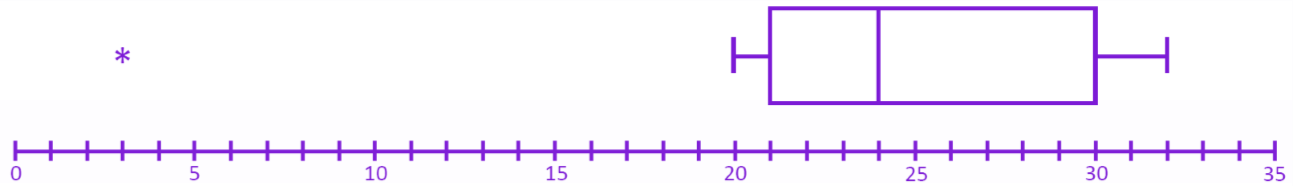
\includegraphics[scale=.7]{STAT_2300_Practice_3-4_3-5_boxplot.png}
			\end{center} 
			\vspace{3mm}		
			
		\end{solution}
		
		\part Describe the \textbf{distribution} of the boxplot you constructed by discussing its shape, center, spread, and any outliers.
		
		\begin{solution}[\stretch{1}]
	
			\vspace{3mm}		
		
			The distribution of bite times is skewed left with one low outlier of 3 minutes. It has a median of 24 minutes and an IQR of 9 minutes.
			
			\vspace{3mm}		
			
		\end{solution}
		
	\end{parts}
	

\end{questions}

%-----------------------------------------------------------------------------%

\end{document}
